\Chapter{RISK-AWARE ROUTING IN ROBOT SWARMS}\label{sec:Theme2}

%Small intro
In this chapter, the paper \textit{RASS: Risk-Aware Swarm Storage} \cite{arseneault2022rass}, to which I contributed as second author in the course of my master's degree, will be presented. RASS has been heavily inspired by DORA-Explorer and similarly to the latter, brings risk-awareness to a robot swarm algorithm. Specifically, RASS makes the following contributions to the field of swarm robotics: A fully decentralized storing and routing algorithm where the decisions made are based solely on local interactions. The absence of central coordination makes it well-suited for robot swarm applications where scalability is at the core of the problem.

The figures presented in the chapter are taken from the article \cite{arseneault2022rass} with permissions from the authors. 


\section{Introduction}
The exploration of unknown environments has proven to be more effective using teams of robots instead of a single robotic unit \cite{burgard2005coordinated}. Search and rescue scenarios \cite{kantor2003search} or nuclear inspection and cleanup \cite{schwagerMultirobotControlPolicy2017}, where speed is of the essence, are therefore well-suited for multi robot applications. However, data storage remains a challenge for such systems as the amount of collected information only increases with the number of robot. The unreliable connectivity that these systems typically suffer from \cite{amigoni2017multirobot} inhibits sending collected data items directly to external storage. Robots often need to store locally the data items until a path towards permanent storage becomes available. Additionally, because robots usually have limited communication range, the data items collected during the mission may need to be routed through multiple robots before reaching the external storage infrastructure. The multi robot system becomes a temporary storage infrastructure and deciding where to store and send the data items becomes essential. Routing the data items through the shortest path towards the base station may seem natural, however because the environment into which the mission is being carried is usually uncontrolled, environmental hazards can compromise some of the nodes of the system. For example, routing information through a robot located nearby a radiation source might cause data corruptions. Avoiding such nodes of the system can effectively increase the reliability of the system, thus risk should be considered when storing and routing data items. We propose a fully decentralized Risk-Aware Swarm Storage (RASS) system that actively routes data items towards a base station while avoiding dangerous nodes of the system. The algorithm relies solely on local interaction to determine which nodes are the fittest for storing information and works in both static and dynamic topologies.


\section{System model}
We consider a multi-robot system exploring an unknown environment in a fully decentralized fashion. The agents of the system, denoted as $a_i \in A$, are assumed to have limited storage capacities and communication capabilities. While exploring the environment, robots keep acquiring new data and try to convey the information to a base station for permanent storage. Because of their limited communication range $R$, robots may not be able to directly send data items to the base station. They might instead need to route the information through multiple robots before reaching the base station. Finally, point radiation sources $S$ with intensities $I_j\sim\mathcal{U}(0, 1)$ are randomly distributed in the environment. We assumed these radiation sources to be the cause of data corruptions on nearby robots \cite{sharp1996radiation,messenger1986effects}.  

The total radiation level perceived by a robot $a_i$ at position $\bm{x}_i \in E$ is given by:

\begin{equation}
    r(\bm{x}_i) = b + \sum_{\bm{s_j} \in S} \frac{I_{\bm{s_j}}}{1 + \lambda\rho(\bm{x}_i)^2}
    \label{eq:radiation}
\end{equation}

The radiation level decays exponentially with the Euclidean distance $\rho(\bm{x}_i)$ between the position of the radiation source $\bm{s}_j$ and the one of the robot $\bm{x}_i$. $\lambda$ is used as a decay rate parameter and Gaussian measurement noise
$b \sim \mathcal{N}(0, 0.05)$ is added to the readings of the on-board sensor. We assume that the radiation sources affect the robots independently and therefore, the probability of data being corrupted follows a Bernoulli distribution and is given by:

\begin{equation}
    \mathbb{P}(c_i = 1 | S) \sim \mathcal{B}(r(\bm{x}_i)) = 1 - \prod_{\bm{s_j} \in S} 1 - \mathbb{P}(c_i = 1 | \bm{s}_j)
    \label{eq:failure}
\end{equation}


RASS is built upon the assumption that nodes of the system exposed to higher level of radiation should be used less in storing and routing data items. Indeed, because radiation is assumed to cause data corruptions, avoiding dangerous locations of the system should offer better reliability results and effectively reduce the number of lost data items. Additionally, to alleviate the memory usage of the robots of the system, percolating data items towards a base station for permanent storage should be encouraged. From this, and taking inspiration from \cite{majcherczykSwarmmesh2020}, we define a fitness policy that indicates how "fit" an agent is for storing data items. The fitness of an agent is given by:

\begin{equation}
        \phi_i =
        \left\{ 
        \begin{array}{ll}
            \frac{1}{\alpha h_i + \beta r({\bm{x}_i})} &\text{if } m_i > 0 \\
            0 &\text{otherwise}
        \end{array} \right.
        \label{equation:fitness}
\end{equation}

where $\alpha$ and $\beta$ are respectively the routing and risk control gains, $m_i$ is the available memory of agent $a_i$,  $r_i$ is the risk given by eq. \ref{eq:radiation} and $h_i$ is the minimum hop count to the base station. When a node becomes unfit to store data items, it will simply evict items to its fittest neighbour:

\begin{equation}
    T\phi_i < \max_{j \in \mathcal{N}} \phi_j
\end{equation}

$\mathcal{N}$ is the set of neighbours of agent $a_i$ and $T$ is a fitness threshold that ensures that data items are routed only when a neighbour is significantly better for storing them. Because of the hop count gain included in the fitness policy, data items will tend to passively percolate towards the base station. Indeed, for similar levels of risk, nodes located closer to the base station should have higher fitness. RASS' execution loop is summarized in algorithm \ref{alg:rass}. 

\begin{algorithm}[h]
\small
\SetAlgoLined
\DontPrintSemicolon
    \While{Running}{
        $get\_hop\_count()$\;
        $get\_risk\_measurement()$\;
        $update\_fitness()$\;
        \;
        \If{not $is\_fit()$ and $|\mathcal{N}| > 0$}{
            $evict\_data()$\;
        }
        \;
    }
 \caption{RASS Execution Loop}
 \label{alg:rass}
\end{algorithm}



\section{Simulations}

To assess the validity of our system, we tested RASS through simulations in the physics-based simulator ARGoS \cite{Pinciroli:SI2012}. The agents used
in the simulation are KheperaIV robots \cite{kteam2021kheperaiv} and RASS' implementation is done using the Buzz programming language from \cite{pinciroliBuzz2016}.

To thoroughly assess RASS' performance, four different robot topologies were studied:

\begin{itemize}
    \item Grid like pattern (static topology) as shown in figure \ref{argos:grid}
    \item Scale-free pattern (static topology) as shown in figure \ref{argos:scale-free}
    \item Lennard-Jones potential interactions (dynamic topology) as shown in figure \ref{argos:lennard-jones}
    \item Random search motions (dynamic topology) as shown in figure \ref{argos:random-walk}
\end{itemize}

\begin{figure}[htbp]
	\centering
    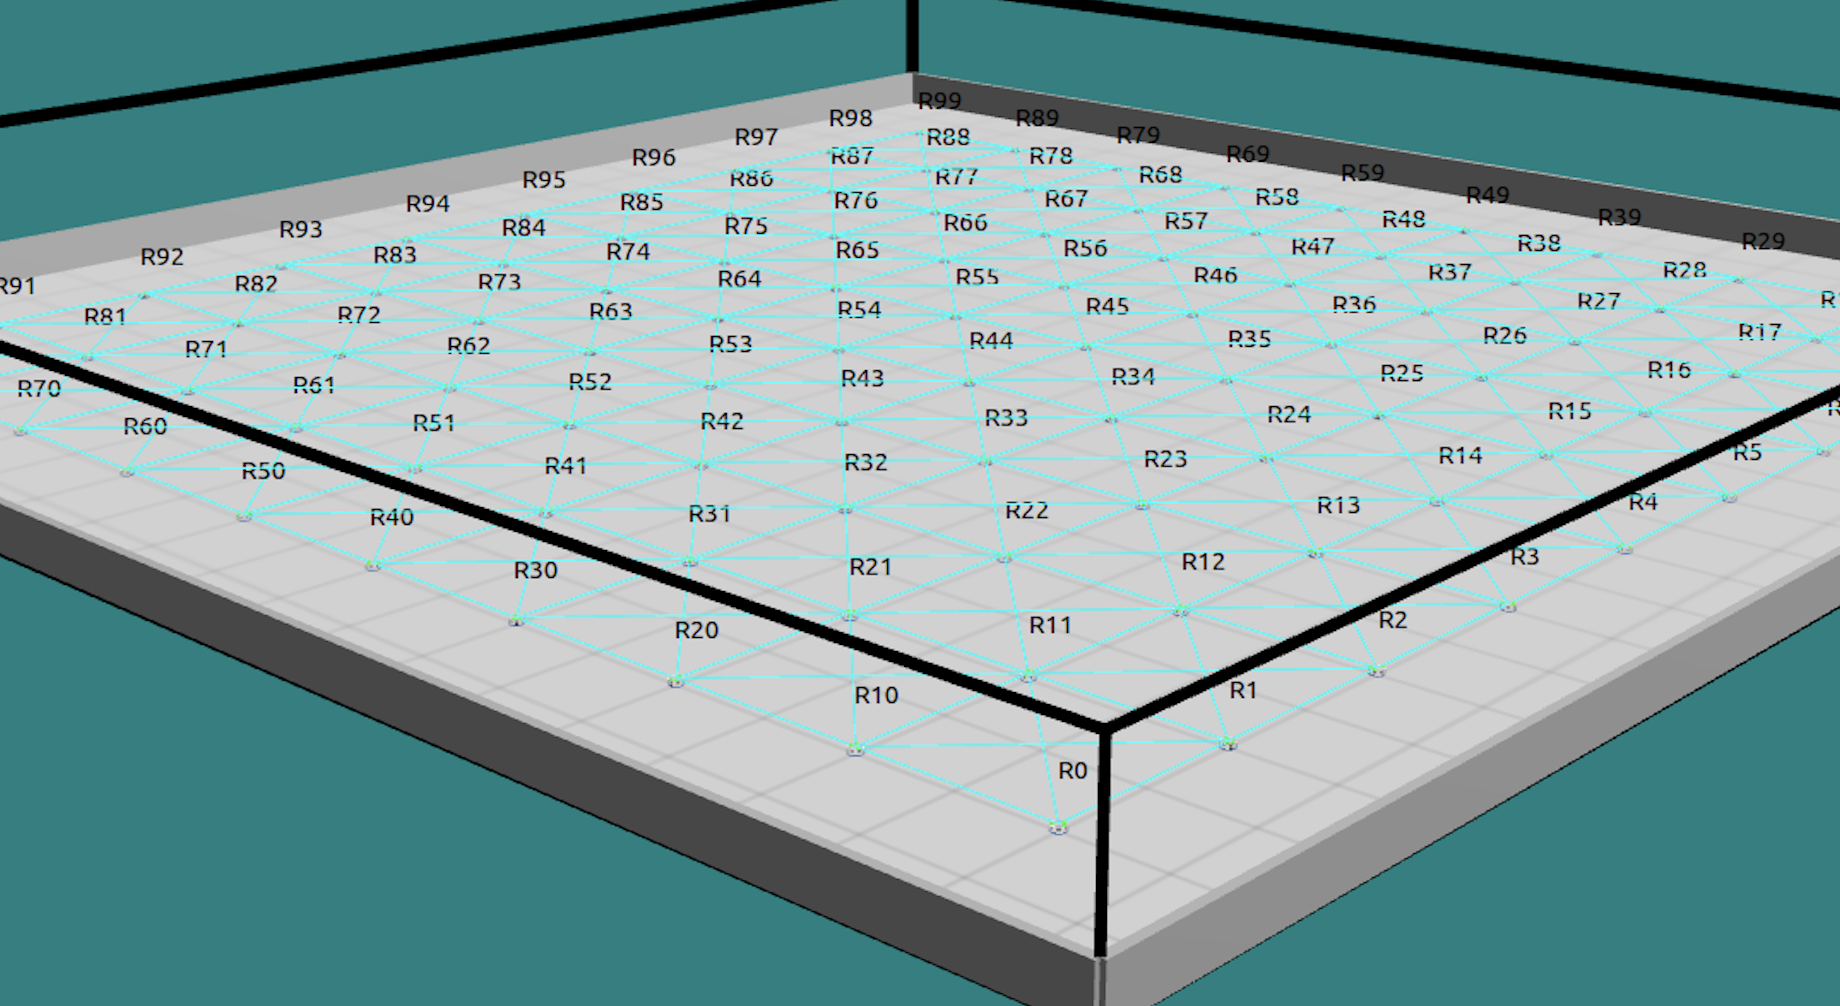
\includegraphics[width=\columnwidth]{images/argos_grid_link.png}
    \caption[Grid formation in ARGoS]{100 KheperaIV robots in 20m x 20m  ARGoS simulated environment distributed in a grid-like pattern.}
    \label{argos:grid}
\end{figure}

\begin{figure}[htbp]
	\centering
    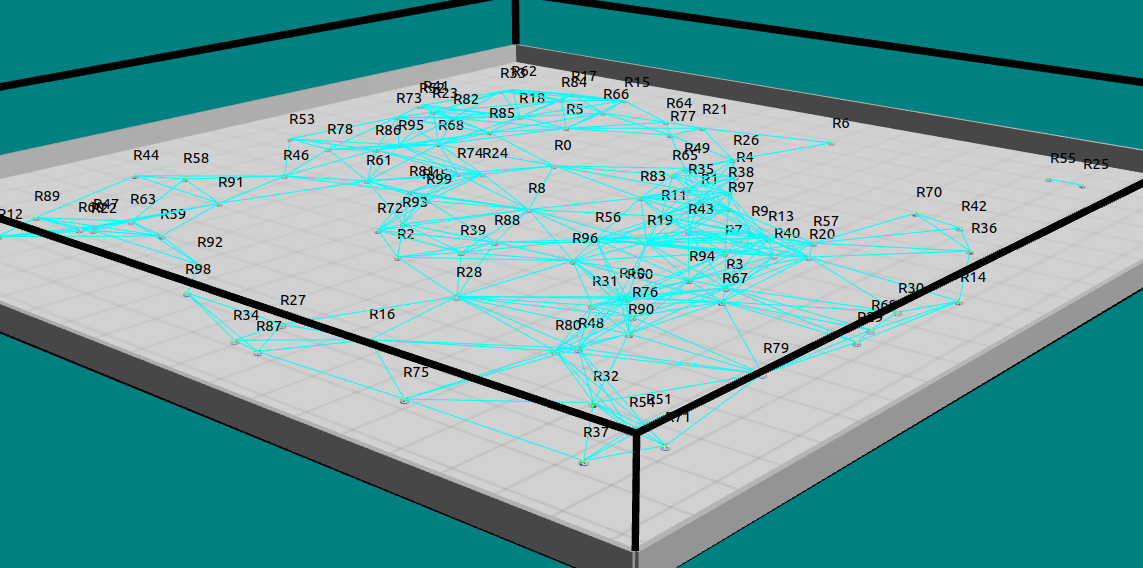
\includegraphics[width=\columnwidth]{images/argos_scale_free.png}
    \caption[Scale-free formation in ARGoS]{100 KheperaIV robots in 20m x 20m  ARGoS simulated environment distributed in a scale-free pattern.}
    \label{argos:scale-free}
\end{figure}

\begin{figure}[htbp]
	\centering
    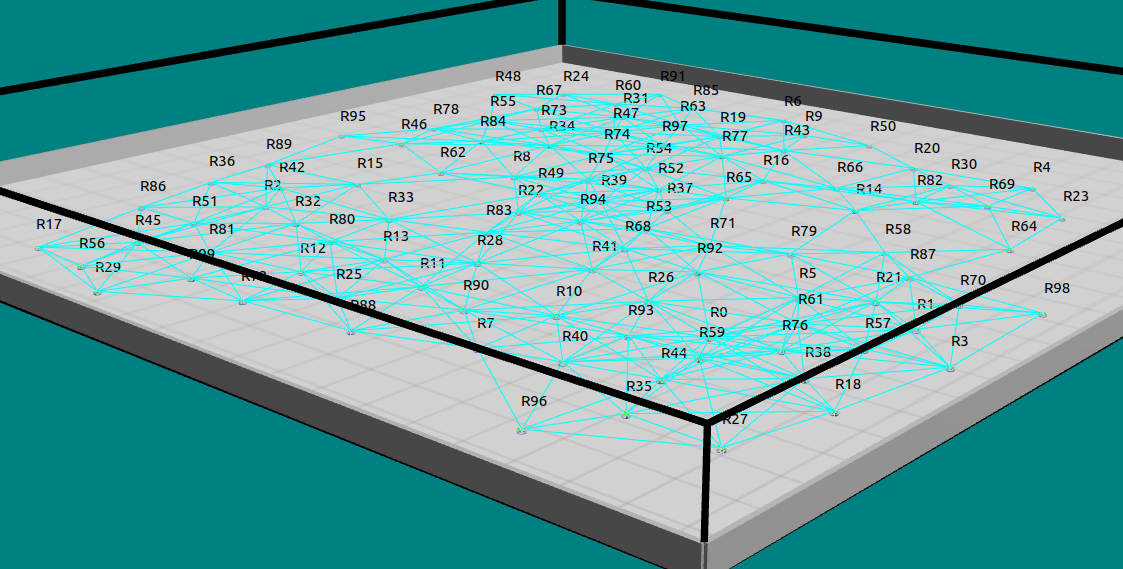
\includegraphics[width=\columnwidth]{images/argos_lennard.png}
    \caption[Lennard-Jones potential formation in ARGoS]{100 KheperaIV robots in 20m x 20m  ARGoS simulated environment in a dynamic topology obtained through Lennard-Jones potential interactions.}
    \label{argos:lennard-jones}
\end{figure}

\begin{figure}[htbp]
	\centering
    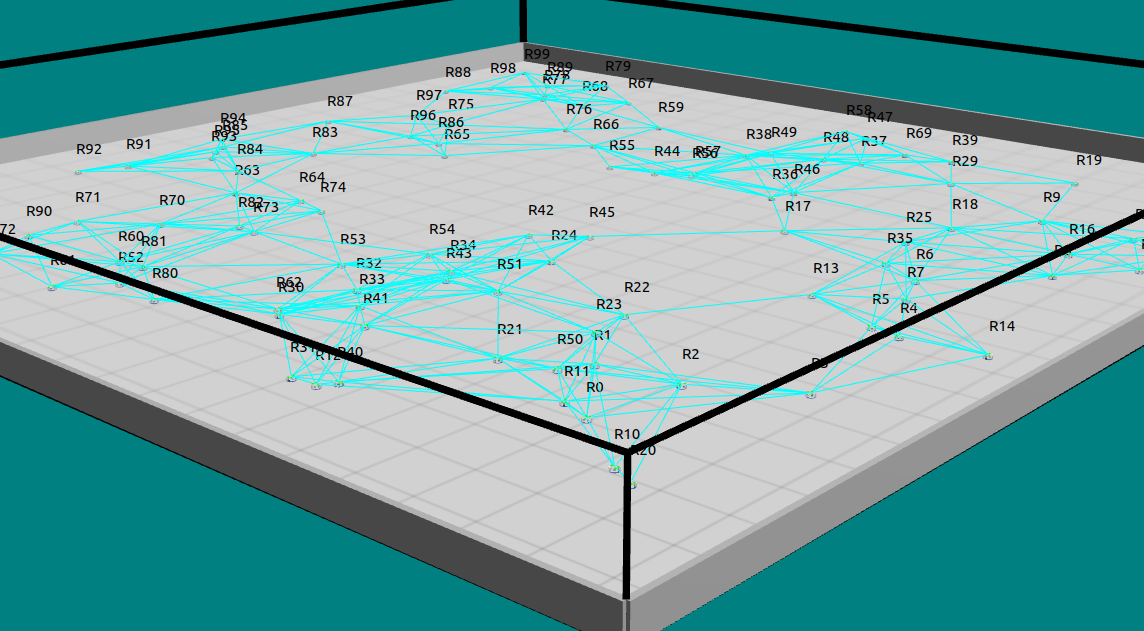
\includegraphics[width=\columnwidth]{images/argos_random.png}
    \caption[Random formation in ARGoS]{100 KheperaIV robots in 20m x 20m  ARGoS simulated environment in a dynamic topology obtained through random walk motions.}
    \label{argos:random-walk}
\end{figure}

We deploy N = 100 robots with a communication radius $R$ = 3 meters in a 20m x 20m environment containing a set of 3 randomly distributed radiation sources. The base station is located in a corner of the environment and its storage capacity is assumed to be infinite. To bring our simulations closer to real world scenarios, we added bandwidth limitations to the amount of data robots can possibly exchange. In our simulations, the maximal number of data items that could be exchanged between two neighbouring robots was 10 items every time step. Data items were generated at a fixed interval by all robots in the system. The storage capacity of robots was set to 50 data items. For our simulations, we used $\alpha = 10$ and $beta = 1$ for Eq. \ref{equation:fitness}. This choice was justified by the fact that the risk $r({x_i})$ was bounded by [0,1] while the hop-count value $h_i$ was not. In our simulations, $h_i$ was usually upper-bounded by 10. Therefore, choosing of value of $\alpha = 10$ gave the two parameters a similar importance when determining the fitness in Eq. \ref{equation:fitness}. Two benchmark algorithms were used to assess RASS' performance:

\begin{itemize}
    \item A routing algorithm based on hop-count 
    \item The virtual stigmergy from \cite{pinciroliTuple2016}
\end{itemize}

The hop-count based algorithm enables comparison with a commonly used routing mechanism meant to yield fast transfer speeds. The virtual stigmergy was chosen to showcase the benefit of percolating data towards a base station.

The results obtained in the simulations for the different topologies are presented in Fig. \ref{results:staticTopology}, \ref{results:staticTopologyScale}, \ref{results:dynamicTopologyLennard} and \ref{results:dynamicTopologyRandom} and in table \ref{table:speed}. They show that RASS persistently outperforms the hop-count based algorithm and the virtual stigmergy in terms of reliability across all four topologies. Indeed, the percentage of retained data for RASS is usually between 80\% and 100\%, meaning that no more than 20\% of generated data items during the experiments are lost due to corruption. On the other hand, the hop-count based algorithm offers reliability results ranging from 50\% to 80\% and is therefore more affected by the radiations sources of the environment. Finally, the virtual stigmergy offers low reliability results as the storage capacity of the agents is quickly saturated and new data items cannot be stored no more. In terms of transfer speeds, results show that the fastest routing mechanism is the hop-count based algorithm. In average, RASS is 54.9\% slower than the hop-count based algorithm, in other words it takes 54.9\% more steps for data items to reach the base station using RASS. This is not surprising as the hop-count based algorithm always takes the fastest route towards the base station, regardless of the risk associated with it. In opposition, RASS takes the route that optimizes both speed and safety. RASS offers better reliability results at the cost of slower transfer speeds.  

\begin{figure*}
    \centering
    \begin{subfigure}{0.8\textwidth}
        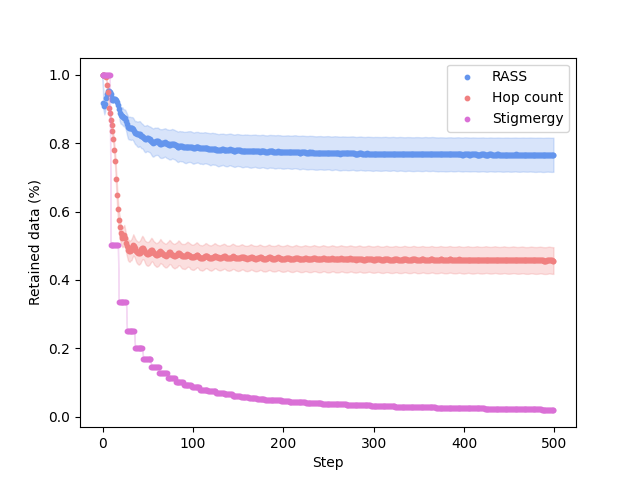
\includegraphics[width=\textwidth]{images/grid_reliability.png}
        \caption{Reliability over time}
        \label{results:grid_100_reliability}
    \end{subfigure}
    \begin{subfigure}{0.8\textwidth}
        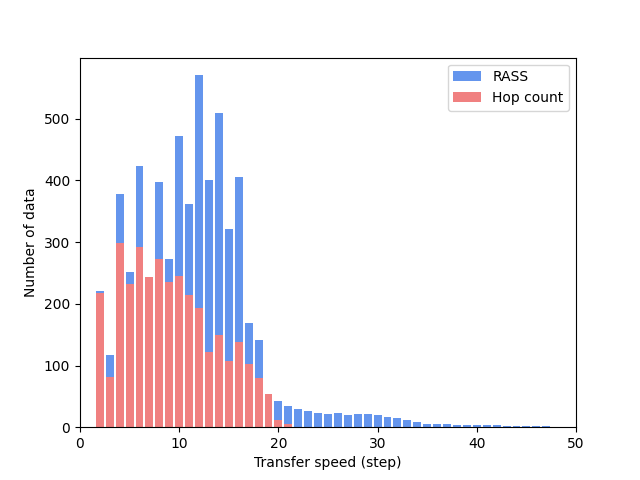
\includegraphics[width=\textwidth]{images/grid_speed.png}
        \caption{Distribution of transfer speeds}
        \label{results:grid_100_speed}
    \end{subfigure}
    \caption{Performance comparison of RASS, hop count and stigmergy in a static grid-like topology.}
    \label{results:staticTopology}
    \vspace{-2mm}
\end{figure*}

\begin{figure*}
    \centering
    \begin{subfigure}{0.8\textwidth}
        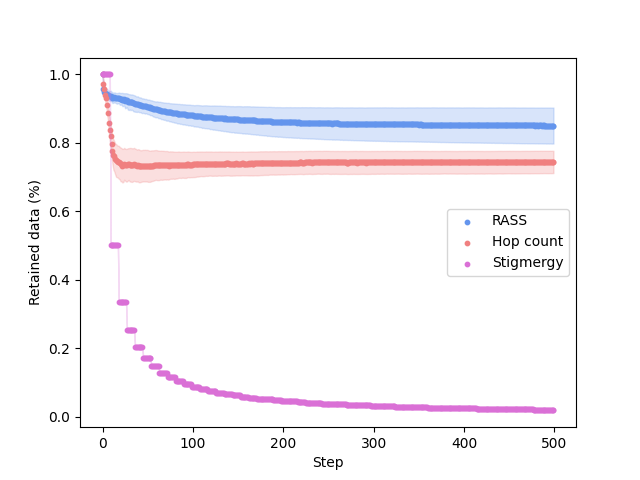
\includegraphics[width=\textwidth]{images/scale_reliability.png}
        \caption{Reliability over time}
        \label{results:scale_100_reliability}
    \end{subfigure}
    \begin{subfigure}{0.8\textwidth}
        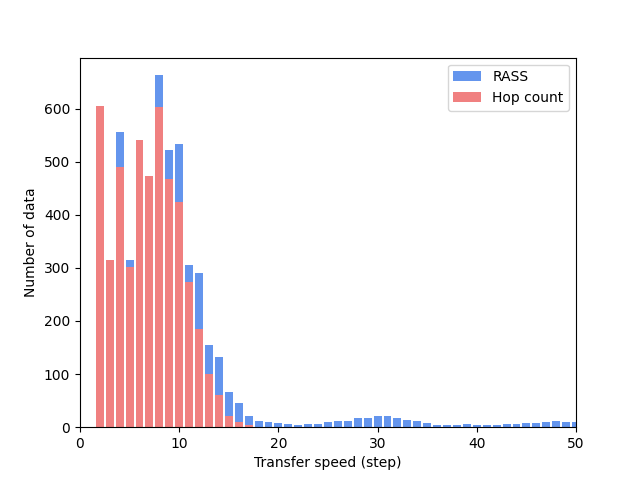
\includegraphics[width=\textwidth]{images/scale_speed.png}
        \caption{Distribution of transfer speeds}
        \label{results:scale_100_speed}
    \end{subfigure}
    \caption{Performance comparison of RASS, hop count and stigmergy in a static Scale Free topology.}
    \label{results:staticTopologyScale}
    \vspace{-2mm}
\end{figure*}

\begin{figure*}
    \centering
    \begin{subfigure}{0.8\textwidth}
        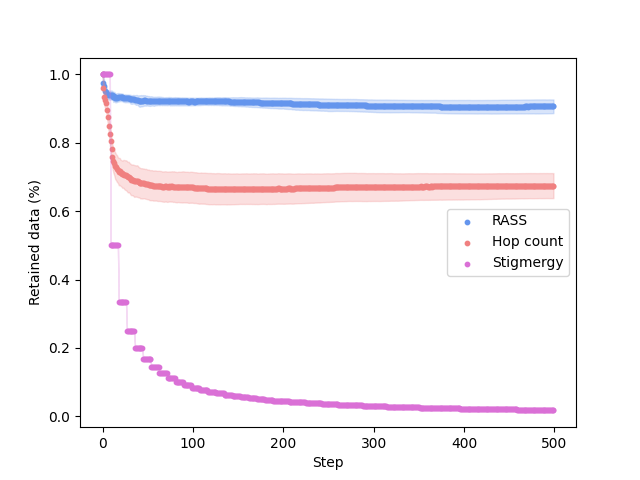
\includegraphics[width=\textwidth]{images/lennard_reliability.png}
        \caption{Reliability over time}
        \label{results:lennard_100_reliability}
    \end{subfigure}
    \begin{subfigure}{0.8\textwidth}
        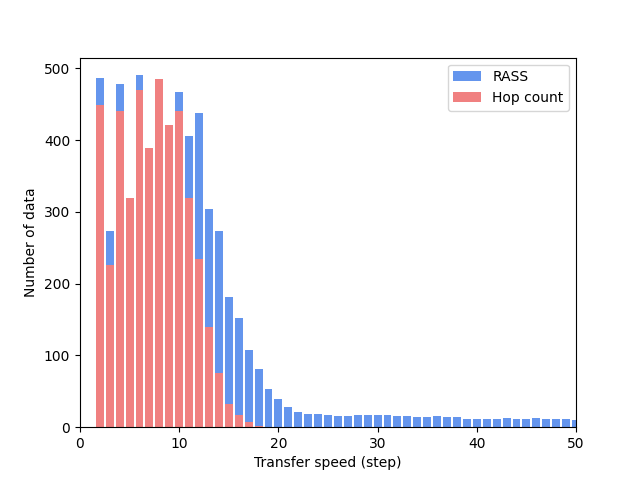
\includegraphics[width=\textwidth]{images/lennard_speed.png}
        \caption{Distribution of transfer speeds}
        \label{results:lennard_100_speed}
    \end{subfigure}
    \caption{Performance comparison of RASS, hop count and stigmergy in a dynamic Lennard-Jones topology.}
    \label{results:dynamicTopologyLennard}
    \vspace{-2mm}
\end{figure*}

\begin{figure*}
    \centering
    \begin{subfigure}{0.8\textwidth}
        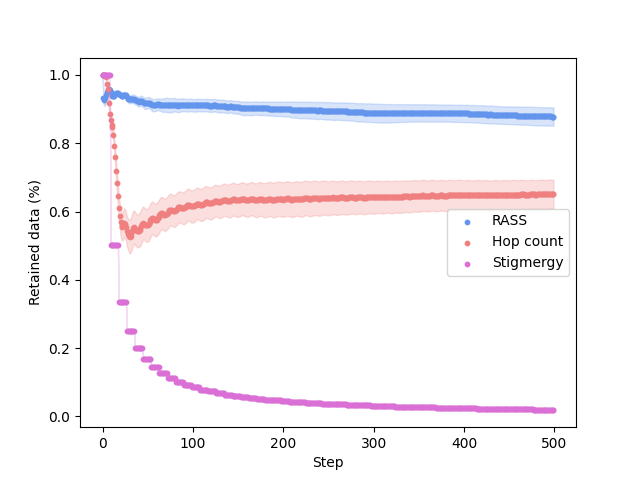
\includegraphics[width=\textwidth]{images/random_reliability.png}
        \caption{Reliability over time}
        \label{results:random_100_reliability}
    \end{subfigure}
    \begin{subfigure}{0.8\textwidth}
        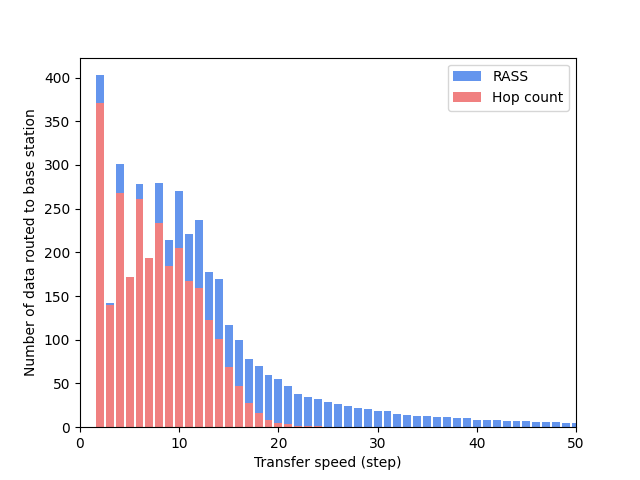
\includegraphics[width=\textwidth]{images/random_speed.png}
        \caption{Distribution of transfer speeds}
        \label{results:random_100_speed}
    \end{subfigure}
    \caption{Performance comparison of RASS, hop count and stigmergy in a dynamic random search topology.}
    \label{results:dynamicTopologyRandom}
    \vspace{-2mm}
\end{figure*}

\begin{table}[]
\centering
\caption{Average transfer speed and average individual memory usage with different topologies}
\label{table:speed}
\def\arraystretch{1.5}
\setlength{\tabcolsep}{8pt}
\begin{tabular}{llcc}
\hline
\multicolumn{1}{c}{\textit{\textbf{Topology}}} &
  \multicolumn{1}{c}{\textit{\textbf{Algorithm}}} &
  \textit{\textbf{\begin{tabular}[c]{@{}c@{}}Transfer speed (hops)\end{tabular}}} \\ \hline
                                         & RASS      & 11.45  \\ \cline{2-3} 
                                         & Hop-Count & 9.11   \\ \cline{2-3} 
\multirow{\textbf{Grid-like}}     & Stigmergy & N.A.  \\ \hline
                                         & RASS      & 11.44    \\ \cline{2-3} 
                                         & Hop-Count & 6.85     \\ \cline{2-3} 
\multirow{\textbf{Scale-Free}}    & Stigmergy & N.A.   \\ \hline
                                         & RASS      & 12.51    \\ \cline{2-3} 
                                         & Hop-Count & 7.32     \\ \cline{2-3} 
\multirow{\textbf{Lennard-Jones}} & Stigmergy & N.A.   \\ \hline
                                         & RASS      & 12.68    \\ \cline{2-3} 
                                         & Hop-Count & 7.76    \\ \cline{2-3} 
\multirow{\textbf{Random Search}} & Stigmergy & N.A.  \\ \hline
\end{tabular}
\end{table}


\section{Physical experiments}

To assess its real-world applicability, we tested RASS with a swarm of 5 physical robots using a static topology illustrated in fig. \ref{cogniflyExperiment1} and fig. \ref{cogniflyExperiment2}. 

\begin{figure}[h]
	\centering
    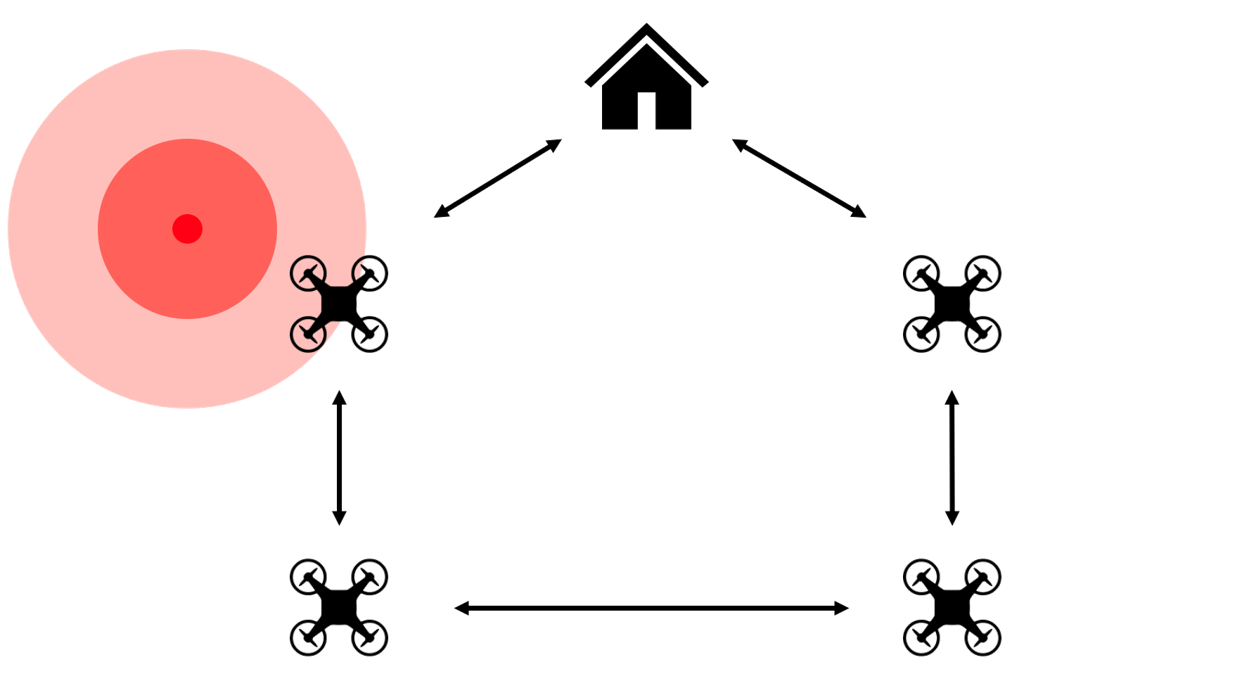
\includegraphics[width=0.7\columnwidth]{images/physical-topology.png}
    \caption{Topology of the 3x3m environment with 4 drones, a base station and a radiation source used in the physical experiments.}
    \label{cogniflyExperiment1}
\end{figure}

\begin{figure}[h]
	\centering
    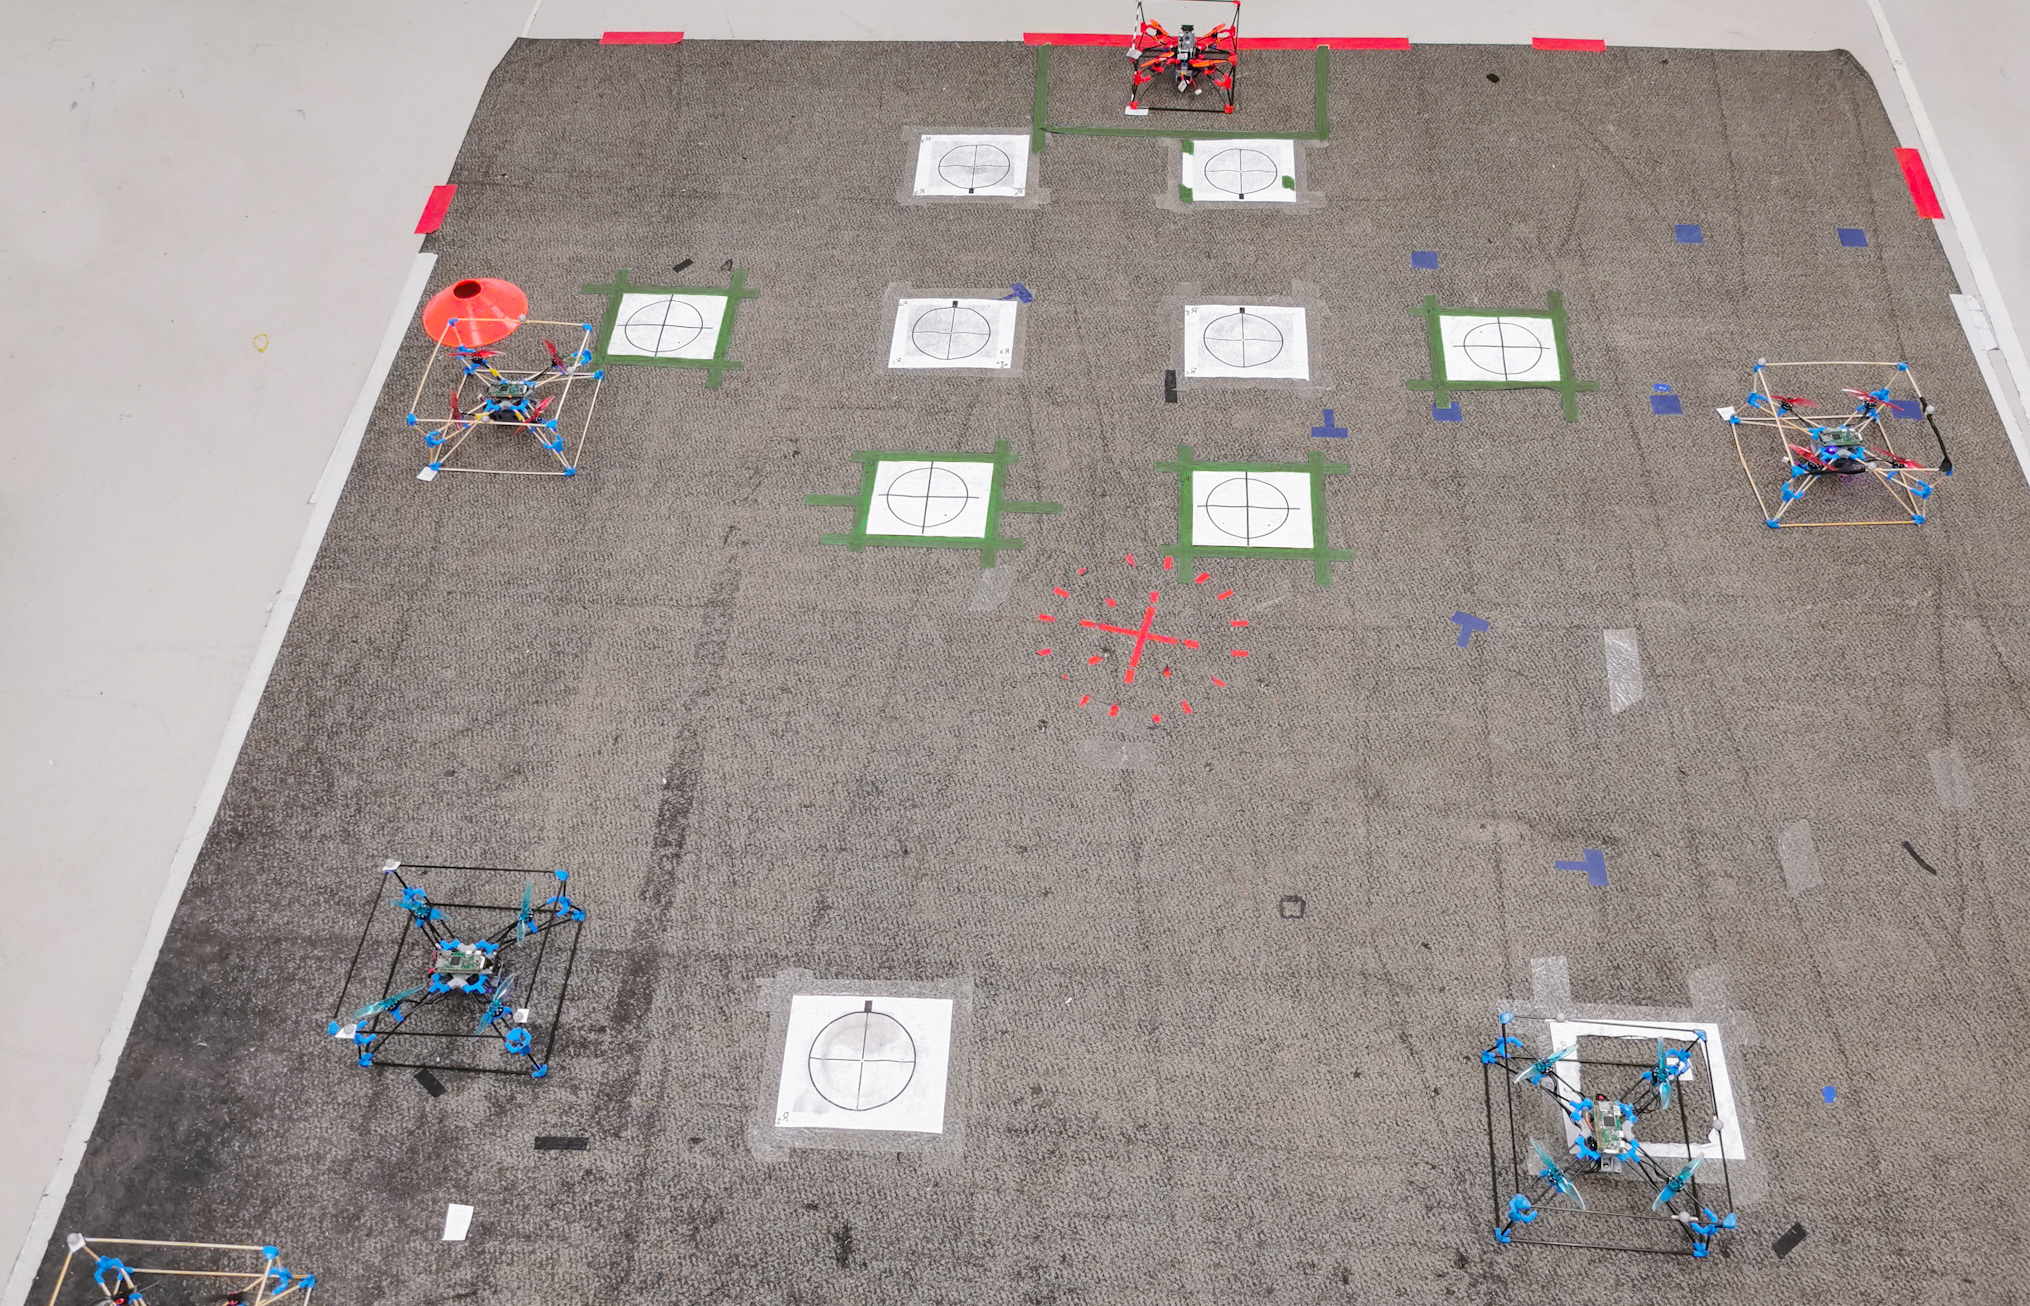
\includegraphics[width=0.64\columnwidth]{images/cognifly.jpg}
    \caption{Picture of the 3x3m environment with 4 drones, a base station and a radiation source used in the physical experiments.}
    \label{cogniflyExperiment2}
\end{figure}

The goal was showing that the algorithm was easily transferable to physical robots and that it behaves the ways it is intended to. In this particular topology, one route is clearer safer than the other. We expect RASS to choose the safest one even if it is not necessarily the fastest one towards the base station. We performed 3 runs of the RASS alogrihm and compared its performance with the hop-count based algorithm. Results are presented in fig. \ref{results:physicalRelaibility}.

\begin{figure}[h]
	\centering
    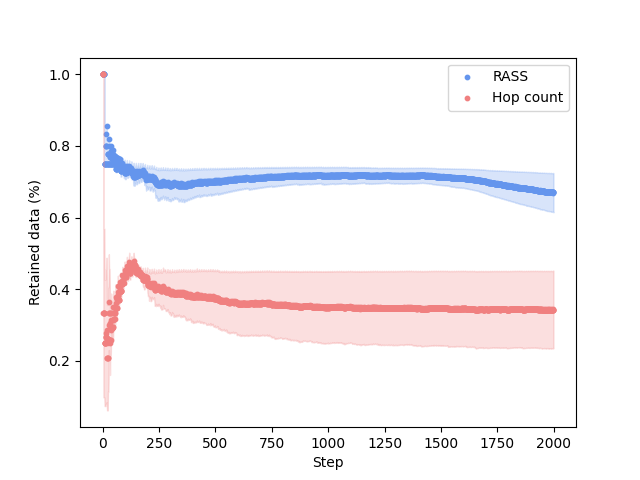
\includegraphics[width=0.90\columnwidth]{images/reliability.png}
    \caption{Evolution of reliability over time on the the physical experiments}
    \label{results:physicalRelaibility}
\end{figure}


Again, results show that RASS offers better reliability results than the hop-count based algorithm. RASS' percentage of retained data is about 75\%, which it what was expected in the particular topology. Indeed, one of the four robots is located on the radiation source and therefore looses almost all its data items due to corruption. The other three robots are able to route their data items using the safe route. On the other hand, the hop-count based algorithm looses a bit more than 50\% of the data items as the two possible routes towards the base station as taken analogously, regardless of the risk. It is true that very few conclusions can be drawn by the physical experiments as the swarm size is very limited and the topology chosen arbitrarily. However, the main motivation was showing that the algorithm, as it is, can be easily implemented on physical robots and can run the way it is intended to. Of course, further physical experiments, with a greater number of robot and more realistic topologies, will need to be carried to assess RASS' performance in real world scenarios.

\section{Conclusion}

We presented RASS, a fully decentralized risk-aware storing and routing algorithm. By leveraging a fitness policy based on both hop-count and risk, RASS is able to choose the appropriate agents through which to route data items towards the base station. Results from our experiments show that RASS consistently outperforms the hop-count based algorithm in terms of reliability across different topologies, both static and dynamic. RASS also performed well in physical experiments where the main motivation was showing that the algorithm, as it is, can be easily implemented on physical robots and can run the way it is intended to.

Additional experiments on larger swarms of robots and in more diverse scenarios will be necessary to assess RASS' performance in real world missions. Also, some additional work include understanding the impact of the communication network assumptions on the performance of RASS. For example, a network where there exists only a few routes towards the base station and where one is clearly safer than the other is of course well-suited for our algorithm. On the other hand, the value of RASS should decrease in well connected networks where the radiation sources are only located at the periphery of the network (far from the base station). Indeed, in this particular scenario, because data naturally moves away from the risk, RASS' risk-awareness shouldn't improve noticeably the network's reliability.

